Este capítulo incidirá sobre o desenvolvimento e implementação da aplicação móvel do nosso projeto. Começaremos por realizar uma pequena introdução, de seguida apresentando a navegação na aplicação e a sua arquitetura, concluindo este capítulo discutindo cada componente da mesma.

\bigskip

\section{\textit{Mobile App}}

O segundo componente deste projeto é a aplicação móvel. Esta funciona como interface para o tipo de utilizador mais comum (Voluntário) e foi desenvolvida para a plataforma Android.

\bigskip

Este módulo contém alguns requisitos chave que são necessários para garantir a usabilidade da mesma por parte dos seus utilizadores. Seguem-se alguns dos requisitos a cumprir diante dos voluntários:

\begin{itemize}
	\item garantir que possam ver os \textit{posts} e eventos que estão registados na plataforma;
	\item possibilitar que possam gostar \textit{posts}, seguir utilizadores e registarem-se em eventos (ou seja, implementar a interação de uma rede social)
	\item existência do conceito sessão de maneira a terem uma experiência personalizada, e possibilitar que possam editar ou seu perfil, efetuar \textit{posts}, entre outros.
\end{itemize}

Tal como já foi referido anteriormente, foi tomada a decisão de implementar esta aplicação no sistema operativo Android seguindo as orientações dadas pelo Android Jetpack e um conjunto de bibliotecas auxiliares (como o Volley e o Glide).

\bigskip

\subsection{Navegabilidade e utilização da \textit{App}}

Tendo em conta que este componente constitui uma interface gráfica (ou seja, irá ser utilizada em primeira instância por utilizadores humanos), existiu durante o desenvolvimento do mesmo um cuidado em termos de navegação e desenho de maneira a tornar a mesma o mais intuitiva possível. 

\bigskip

De seguida, encontra-se o padrão de navegação definido na figura 7.

\newpage

\begin{figure}[h]
	\centering
	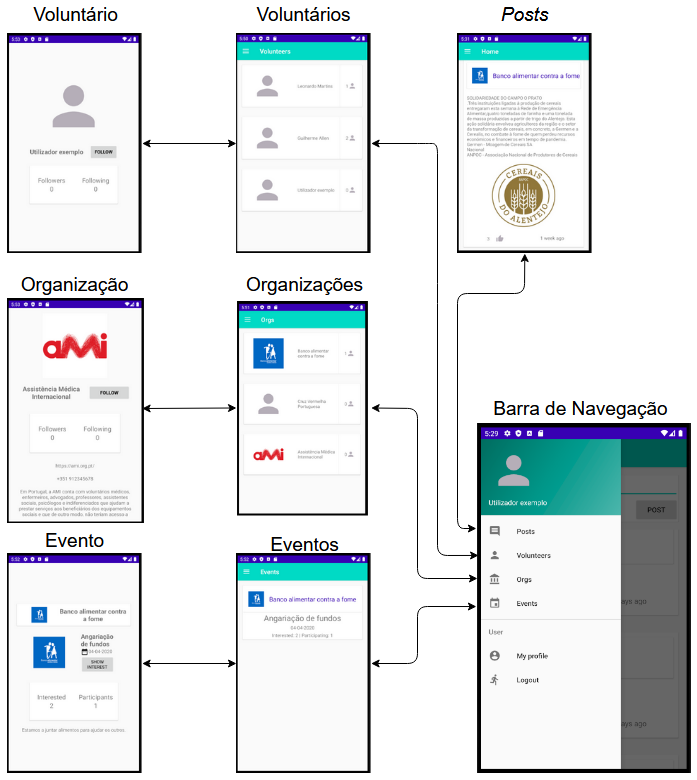
\includegraphics[scale=.55]{app_navigation.png}
	\caption{Grafo de navegação}
\end{figure}

Foram desenvolvidas 4 vistas principais de pesquisa (\textit{posts}, voluntários, organizações e eventos) de maneira a apresentar os dados na plataforma já existentes e também vistas detalhadas para estes mesmos índices (excepto \textit{posts}) para que o utilizador pudesse ver os detalhes destes dados.

\bigskip

\subsection{Sessão}

De maneira a garantir uma experiência personalizada para cada cliente deste módulo, foram desenvolvidos ecrãs e mecanismos de maneira a que clientes do mesmo se possam registar/autenticar.

\bigskip

A partir do momento que um cliente da aplicação se encontre autenticado, certas operações como "gostar" um \textit{post} ou seguir um utilizador passam a estar disponíveis e determinados ecrãs iram ter uma vista personalizada, tal como exemplificado na figura 8.

\newpage

\begin{figure}[h]
	\centering
	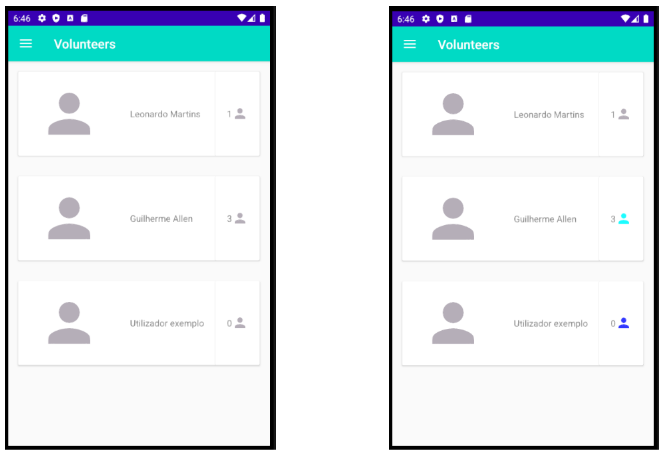
\includegraphics[scale=.70]{unauthenticated_vs_authenticated}
	\caption{Representação do ecrã ''Voluntários'' no estado não autenticado (figura da esquerda) \textit{versus} no estado autenticado como o utilizador "Utilizador exemplo" (figura da direita)}
\end{figure}

\subsection{Arquitetura}

A arquitetura da aplicação é constituída por 3 sub-módulos principais: UI (User Interface), API e Modelo.

\medskip

Enquanto que a UI é responsável por conter as implementações dos mais variados aspetos da interface de utilizador (como atividades, fragmentos, navegação e outros elementos), a API trata a comunicação entre a aplicação e a Web API do projeto. Por fim, o Modelo define a estrutura dos dados fornecidos pela API e utilizados na UI assim como a implementação de uma \textit{cache} de maneira a partilhar estes mesmos dados e reduzir o número de pedidos efetuados à Web API.

\subsection{Sessão}

Tendo em conta que o conceito de sessão foi implementado na Web API através da tecnologia Passport.js (que funciona à base de \textit{cookies}), foi necessário redefinir algumas infra-estruturas da biblioteca Volley (utilizada para efetuar pedidos HTTP) de maneira a que, quando o utilizador estivesses autenticado na aplicação, os pedidos efetuados pela mesma tivessem a informação necessária para a Web API conseguir reconhecer o utilizador.

\medskip

De maneira a que a representação dos vários ecrãs da aplicação seja dinâmica consoante a sessão do utilizador, é definido e utilizado um objeto Sessão, acessível por todas as classes do projeto, cujo contém informações relativamente ao voluntário autenticado.

\subsection{\textit{User Interface}}

Este sub-módulo engloba todos os componentes do projeto que são responsáveis por representar os dados da aplicação, sendo que não são efetuadas alterações na interface de utilizador noutros módulos. Como tal, este é constituído por:

\begin{itemize}
	\item implementações de ecrãs, quer sejam atividades ou fragmentos. É de notar que para cada um destes existe um objeto ViewModel associado, responsável por manter o estado dos elementos do ecrã e também por interagir com a API quando necessário; 
	\item adaptadores. Estes são utilizados pelos ecrãs quando existe a necessidade de apresentar uma lista de elementos (como voluntários ou \textit{posts}) tomando proveito do componente RecyclerView;
	\item Outros componentes utilitários, como por exemplo uma estrutura que auxilia o carregamento de imagens para a representação das mesmas.
\end{itemize} 

\subsection{API}

O sub-módulo API (figura 9) serve como \textit{proxy} entre a aplicação e a Web API. Este dispõe de um serviço que disponibiliza todas as rotas acessíveis pelos voluntários e sobre o mesmo é possível solicitar a realização de pedidos à API (como a obtenção de voluntários ou o seguimento, por parte do utilizador autenticado, de uma organização). O mesmo é assíncrono e funciona à base de \textit{callbacks}.

\begin{figure}[h]
	\centering
	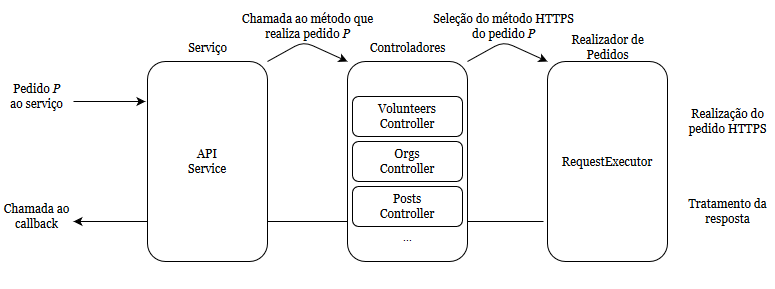
\includegraphics[scale=.42]{mobile_api_architeture}
	\caption{Arquitetura do sub-módulo API}
\end{figure}

O realizador de pedidos trata da implementação dos métodos HTTP suportados pela Web API (GET, POST, PUT, DELETE) de forma genérica, de maneira a que o mesmo possa ser utilizado pelos controladores.

Quando o pedido é concluído, é chamado o \textit{callback} definido pela estrutura que chamou o serviço, que consume a resposta do mesmo, quer esta contenha dados ou apenas sinalize sucesso. A estrutura que efetua a chamada ao serviço é também responsável por definir o \textit{callback} a executar em caso de ocorrer um erro durante o pedido.

\subsection{Modelo}

(explicar utilização e implementação)

